\documentclass[11pt,a4paper]{article}

\usepackage[T1]{fontenc}
\usepackage[utf8]{inputenc}
\usepackage[brazil]{babel}
\usepackage{lmodern}
\usepackage{microtype}
\usepackage[margin=2.5cm]{geometry}
\usepackage{amsmath}
\usepackage{graphicx}
\usepackage{booktabs}
\usepackage{float}
\usepackage{caption}
\usepackage[table]{xcolor}
\usepackage{siunitx}
\usepackage[hidelinks]{hyperref}

\sisetup{output-decimal-marker={,}, group-separator={.}, group-minimum-digits=4}
\captionsetup{font=small, labelfont=bf}

% figures produced by src/run_experiments.py and src/plot_samples.py
\graphicspath{{../results_final/}{../results/}}

\newcommand{\code}[1]{\texttt{#1}}

\title{Classificação de imagens do CIFAR-10 com redes \\ convolucionais (CNN) e perceptrons multicamadas (MLP)}
\author{gbonavina}
\date{\today}

\begin{document}
\maketitle

\begin{abstract}
Este relatório avalia 13 redes neurais na classificação das 10 classes do CIFAR-10:
nove redes convolucionais (CNN), que variam profundidade, largura, tamanho do kernel e
hiperparâmetros de treino, e quatro perceptrons multicamadas (MLP). A melhor CNN, com
quatro camadas convolucionais e \num{1686794} parâmetros, atingiu \SI{91,14}{\percent} de
acurácia no conjunto de teste. A segunda melhor (cinco camadas convolucionais) atingiu
\SI{89,60}{\percent}; a diferença de \num{1,54} pontos é estatisticamente significativa
(teste de McNemar, $p \approx \num{2e-8}$). O melhor MLP, mesmo treinado por 400 épocas,
chegou a \SI{69,82}{\percent} com \num{3844682} parâmetros: 21 pontos abaixo da melhor
CNN, usando 2,3 vezes mais parâmetros.
\end{abstract}

% ---------------------------------------------------------------------------
\section{Introdução}

O CIFAR-10 é um conjunto de imagens coloridas pequenas, muito usado para comparar
arquiteturas de redes neurais. Este trabalho tem três objetivos:
\begin{enumerate}
  \item avaliar diferentes topologias e hiperparâmetros de CNN e de MLP;
  \item comparar os dois melhores modelos por meio de suas matrizes de confusão e de um
        teste estatístico pareado;
  \item comparar a melhor CNN com o melhor MLP em acurácia e número de parâmetros.
\end{enumerate}

% ---------------------------------------------------------------------------
\section{Conjunto de dados}

O CIFAR-10 tem \num{60000} imagens RGB de $32\times32$ pixels, divididas igualmente em 10
classes: \textit{airplane}, \textit{automobile}, \textit{bird}, \textit{cat},
\textit{deer}, \textit{dog}, \textit{frog}, \textit{horse}, \textit{ship} e
\textit{truck}. A divisão oficial tem \num{50000} imagens de treino e \num{10000} de teste
(\num{1000} por classe). A Figura~\ref{fig:amostras} mostra um exemplo de cada classe.

\begin{figure}[H]
  \centering
  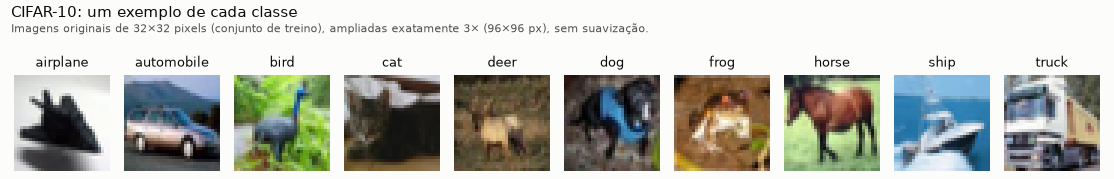
\includegraphics[width=\textwidth]{samples_per_class_compact.png}
  \caption{Um exemplo de cada classe do CIFAR-10, ampliado três vezes sem suavização.
           A baixa resolução torna algumas classes (como \textit{cat} e \textit{dog})
           difíceis de distinguir até para humanos.}
  \label{fig:amostras}
\end{figure}

% ---------------------------------------------------------------------------
\section{Metodologia}

\subsection{Divisão dos dados}

As \num{50000} imagens de treino oficiais foram embaralhadas com semente fixa e divididas
em \num{45000} para treino e \num{5000} para validação. As \num{10000} imagens de teste
oficiais foram mantidas separadas. A mesma divisão foi usada em todos os modelos, o que
permite comparações pareadas.

\begin{itemize}
  \item \textbf{Treino} (\num{45000}): ajuste dos pesos.
  \item \textbf{Validação} (\num{5000}): curvas de aprendizado e escolha dos melhores
        modelos (\textit{ranking}).
  \item \textbf{Teste} (\num{10000}): somente para os resultados finais. Nenhuma decisão
        (escolha de modelo, parada de treino) usa o conjunto de teste.
\end{itemize}

Em todos os casos foi usado o modelo da última época, sem parada antecipada.

\subsection{Pré-processamento e aumento de dados}

Os pixels foram escalados para $[0,1]$ e padronizados por canal com a média
$(0{,}4914;\ 0{,}4822;\ 0{,}4465)$ e o desvio-padrão $(0{,}2470;\ 0{,}2435;\ 0{,}2616)$ do
CIFAR-10. Durante o treino (e apenas no treino) foi aplicado aumento de dados em cada
imagem: espelhamento horizontal com probabilidade \num{0,5} e recorte aleatório de
$32\times32$ após \textit{padding} de 4 pixels, o que desloca a imagem em até $\pm4$
pixels. Todos os modelos usaram aumento de dados, exceto \code{cnn\_4conv\_noaug}, que
serve para medir seu efeito.

\subsection{Arquiteturas}

\paragraph{CNN.} Cada camada convolucional é seguida de \textit{batch normalization},
ReLU e \textit{max pooling} $2\times2$. O número de canais começa em $C$ (largura base) e
dobra a cada camada; o \textit{padding} mantém o tamanho espacial antes do
\textit{pooling}. Após as convoluções, um \textit{global average pooling} reduz cada mapa a
um valor, seguido de um classificador
$\text{Linear}(C_L \to C_L/2) \to \text{ReLU} \to \text{Dropout} \to \text{Linear}(C_L/2 \to 10)$,
em que $C_L$ é o número de canais da última camada.

\paragraph{MLP.} A imagem é achatada em um vetor de \num{3072} valores
($3\times32\times32$), seguido de $L$ camadas ocultas $\text{Linear} \to \text{ReLU} \to
\text{Dropout}$ e de uma camada de saída com 10 neurônios.

As duas redes devolvem \textit{logits}, usados com a função de perda de entropia cruzada.
A Tabela~\ref{tab:configs} lista as 13 configurações avaliadas.

\begin{table}[H]
  \centering
  \small
  \caption{Configurações avaliadas. Salvo indicação, as CNNs usam kernel $3\times3$,
           largura base $C=32$ e \textit{dropout} \num{0,5}; os MLPs usam \textit{dropout}
           \num{0,5}.}
  \label{tab:configs}
  \begin{tabular}{llr}
    \toprule
    Modelo & Descrição & Parâmetros \\
    \midrule
    \code{cnn\_2conv}        & 2 camadas conv. (32, 64 canais)                & \num{21994} \\
    \code{cnn\_3conv}        & 3 camadas conv. (32 a 128 canais)              & \num{102602} \\
    \code{cnn\_4conv}        & 4 camadas conv. (32 a 256 canais)              & \num{423562} \\
    \code{cnn\_5conv}        & 5 camadas conv. (32 a 512 canais)              & \num{1704458} \\
    \code{cnn\_3conv\_k5}    & 3 camadas conv., kernel $5\times5$              & \num{267978} \\
    \code{cnn\_4conv\_w64}   & 4 camadas conv., largura base $C=64$ (64 a 512) & \num{1686794} \\
    \code{cnn\_4conv\_nodrop}& como \code{cnn\_4conv}, sem \textit{dropout}   & \num{423562} \\
    \code{cnn\_4conv\_adamw} & como \code{cnn\_4conv}, otimizador AdamW        & \num{423562} \\
    \code{cnn\_4conv\_noaug} & como \code{cnn\_4conv}, sem aumento de dados   & \num{423562} \\
    \midrule
    \code{mlp\_1x512}        & 1 camada oculta (512)                          & \num{1578506} \\
    \code{mlp\_3\_1024-256}  & 3 camadas ocultas (\num{1024}, 512, 256)       & \num{3805450} \\
    \code{mlp\_2x2048}       & 2 camadas ocultas (\num{2048}, \num{2048})     & \num{10510346} \\
    \code{mlp\_5\_1024-64}   & 5 camadas ocultas (\num{1024} a 64), \textit{dropout} \num{0,2} & \num{3844682} \\
    \bottomrule
  \end{tabular}
\end{table}

\subsection{Treinamento}

Todos os modelos foram treinados com \textit{batch} de 128 imagens e política de taxa de
aprendizado \textit{one-cycle}, que sobe até a taxa máxima e depois decai até quase zero ao
longo de todo o treino. O otimizador padrão foi SGD com \textit{momentum} de Nesterov
(\num{0,9}) e \textit{weight decay} de \num{5e-4}, com taxa máxima de \num{0,05} para as
CNNs e \num{0,01} para os MLPs. O modelo \code{cnn\_4conv\_adamw} usou AdamW com taxa
máxima de \num{2e-3} e \textit{weight decay} de \num{0,05}.

As CNNs foram treinadas por 90 épocas. Os MLPs foram treinados por 400 épocas, porque com
90 épocas a perda de validação ainda caía de forma clara (Seção~\ref{sec:epocas}). Assim,
cada arquitetura foi treinada até próximo da convergência. Os experimentos rodaram em uma
GPU NVIDIA RTX A6000 com PyTorch.

\subsection{Comparação estatística}

Para comparar dois modelos no mesmo conjunto de teste, foi usado o teste exato de McNemar.
Sejam $b$ o número de imagens que só o modelo A acerta e $c$ o número que só o modelo B
acerta. Sob a hipótese nula de desempenho igual, $\min(b,c)$ segue uma distribuição
binomial com $n=b+c$ e $p=0{,}5$. Também foi calculado um intervalo de confiança de
\SI{95}{\percent} para a diferença de acurácia, por \textit{bootstrap} pareado com
\num{2000} reamostragens.

% ---------------------------------------------------------------------------
\section{Resultados}

\subsection{Comparação das topologias}

A Tabela~\ref{tab:ranking} mostra os 13 modelos ordenados pela acurácia de validação.

\begin{table}[H]
  \centering
  \small
  \caption{Resultados ordenados pela acurácia de validação. A acurácia de treino foi medida
           durante a época, com aumento de dados e \textit{dropout} ativos, e por isso pode
           ficar abaixo da de validação.}
  \label{tab:ranking}
  \setlength{\tabcolsep}{4pt}
  \begin{tabular}{rllrrrrrr}
    \toprule
    \# & Modelo & Tipo & Parâmetros & Épocas & Val. (\%) & Teste (\%) & Treino (\%) & Tempo (s) \\
    \midrule
     1 & \code{cnn\_4conv\_w64}    & CNN & \num{1686794}  & 90  & \textbf{91,30} & \textbf{91,14} & 99,03 & 302 \\
     2 & \code{cnn\_5conv}         & CNN & \num{1704458}  & 90  & 91,04 & 89,60 & 97,96 & 346 \\
     3 & \code{cnn\_4conv}         & CNN & \num{423562}   & 90  & 90,42 & 89,54 & 95,65 & 316 \\
     4 & \code{cnn\_4conv\_nodrop} & CNN & \num{423562}   & 90  & 90,04 & 89,41 & 97,24 & 295 \\
     5 & \code{cnn\_4conv\_adamw}  & CNN & \num{423562}   & 90  & 89,86 & 89,05 & 96,94 & 296 \\
     6 & \code{cnn\_3conv\_k5}     & CNN & \num{267978}   & 90  & 87,12 & 86,83 & 90,95 & 179 \\
     7 & \code{cnn\_3conv}         & CNN & \num{102602}   & 90  & 85,68 & 85,54 & 86,37 & 281 \\
     8 & \code{cnn\_4conv\_noaug}  & CNN & \num{423562}   & 90  & 84,02 & 83,75 & 99,99 & 269 \\
     9 & \code{mlp\_5\_1024-64}    & MLP & \num{3844682}  & 400 & 71,64 & 69,82 & 72,56 & 1032 \\
    10 & \code{cnn\_2conv}         & CNN & \num{21994}    & 90  & 70,46 & 69,23 & 64,00 & 251 \\
    11 & \code{mlp\_2x2048}        & MLP & \num{10510346} & 400 & 68,56 & 68,34 & 67,14 & 808 \\
    12 & \code{mlp\_3\_1024-256}   & MLP & \num{3805450}  & 400 & 65,56 & 64,96 & 59,34 & 831 \\
    13 & \code{mlp\_1x512}         & MLP & \num{1578506}  & 400 & 59,94 & 59,94 & 54,04 & 608 \\
    \bottomrule
  \end{tabular}
\end{table}

Os principais efeitos observados nas CNNs foram:
\begin{itemize}
  \item \textbf{Profundidade.} Mais camadas melhoram muito a acurácia até quatro camadas
        (de \SI{69,2}{\percent} com duas para \SI{89,5}{\percent} com quatro). A quinta
        camada praticamente não ajuda (\SI{89,6}{\percent}) e quadruplica o número de
        parâmetros.
  \item \textbf{Largura.} Dobrar a largura da rede de quatro camadas
        (\code{cnn\_4conv\_w64}) deu o melhor resultado (\SI{91,1}{\percent}). Com quase o
        mesmo número de parâmetros, a rede de 4 camadas mais larga superou a de 5 camadas
        mais estreita.
  \item \textbf{Kernel.} O kernel $5\times5$ melhorou a rede de três camadas
        (\SI{85,5}{\percent} para \SI{86,8}{\percent}), ao custo de 2,6 vezes mais
        parâmetros.
  \item \textbf{\textit{Dropout} e otimizador.} Remover o \textit{dropout} ou trocar SGD por
        AdamW mudou o resultado em menos de \num{0,5} ponto: com aumento de dados e
        \textit{batch normalization}, esses hiperparâmetros têm pouco efeito.
  \item \textbf{Aumento de dados.} Foi o fator de treino mais importante. Sem ele, a mesma
        rede caiu de \SI{89,5}{\percent} para \SI{83,8}{\percent}.
\end{itemize}

A Figura~\ref{fig:loss} mostra as curvas de perda. O sobreajuste de
\code{cnn\_4conv\_noaug} é claro: a perda de treino vai a praticamente zero
(\SI{99,99}{\percent} de acurácia de treino), enquanto a perda de validação estaciona em
torno de \num{0,6} a \num{0,8}, com muita oscilação. Nas demais CNNs, as duas curvas
descem juntas por mais tempo e a perda de validação termina entre \num{0,30} e
\num{0,40}.

\begin{figure}[H]
  \centering
  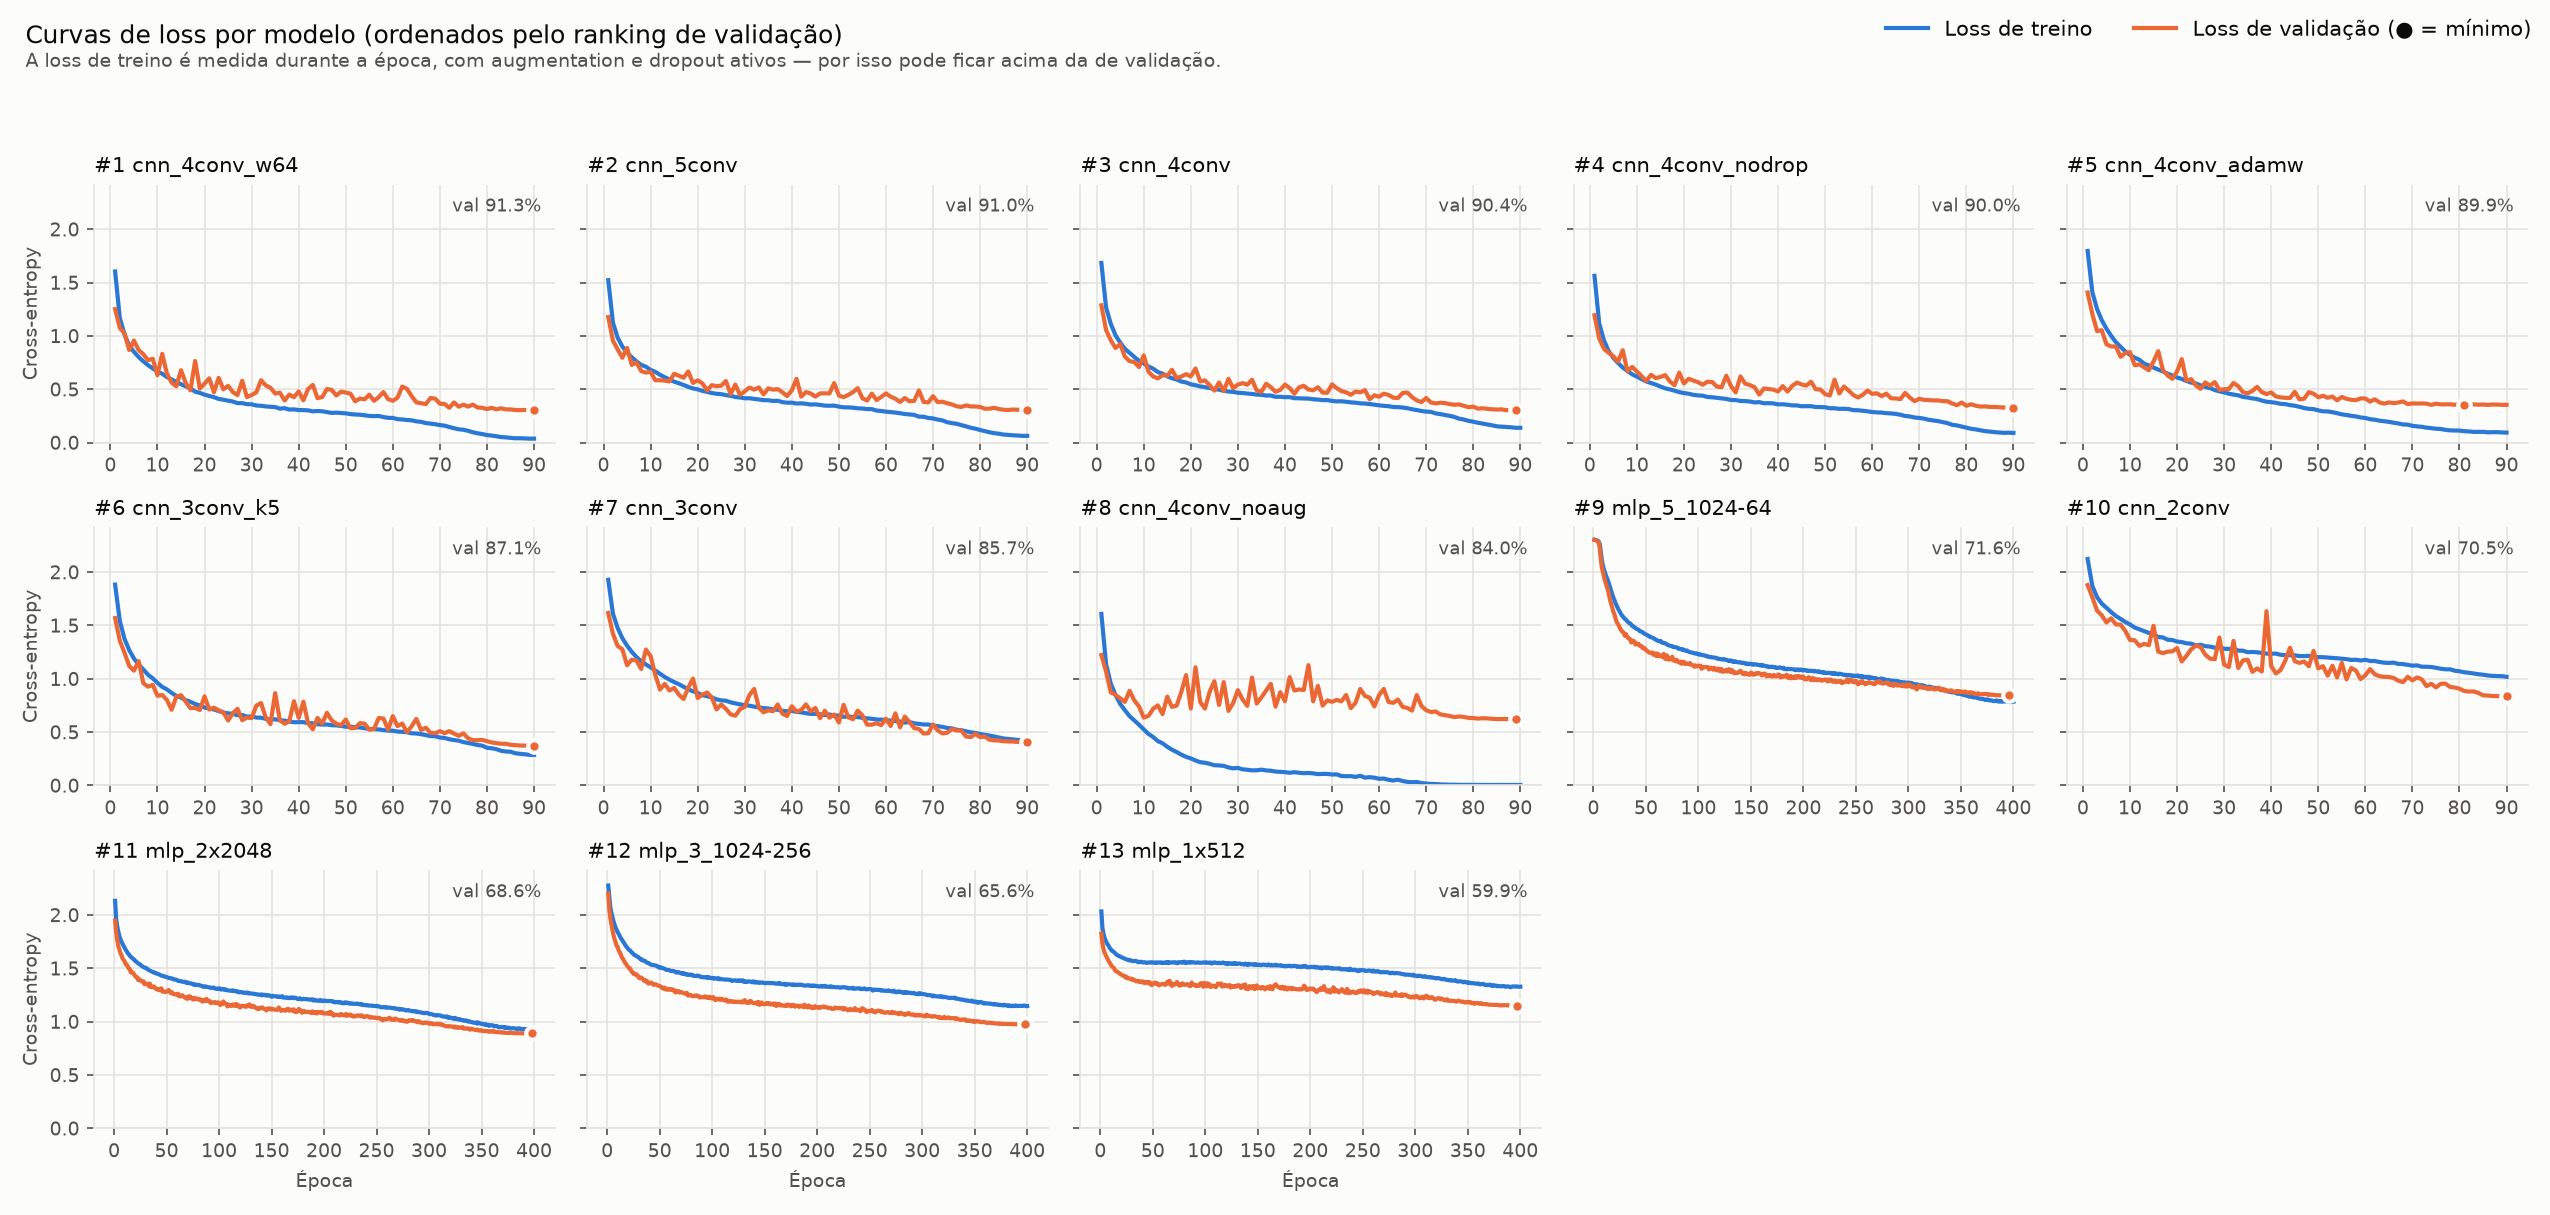
\includegraphics[width=\textwidth]{loss_curves.png}
  \caption{Perda de treino e de validação por época, para cada modelo, na ordem do
           \textit{ranking}. O ponto marca o mínimo da perda de validação. Os MLPs foram
           treinados por 400 épocas e as CNNs por 90, por isso o eixo horizontal varia.}
  \label{fig:loss}
\end{figure}

\subsection{Os dois melhores modelos}

Os dois melhores modelos na validação foram \code{cnn\_4conv\_w64} e \code{cnn\_5conv}. A
Figura~\ref{fig:confusao} mostra suas matrizes de confusão no conjunto de teste.

\begin{figure}[H]
  \centering
  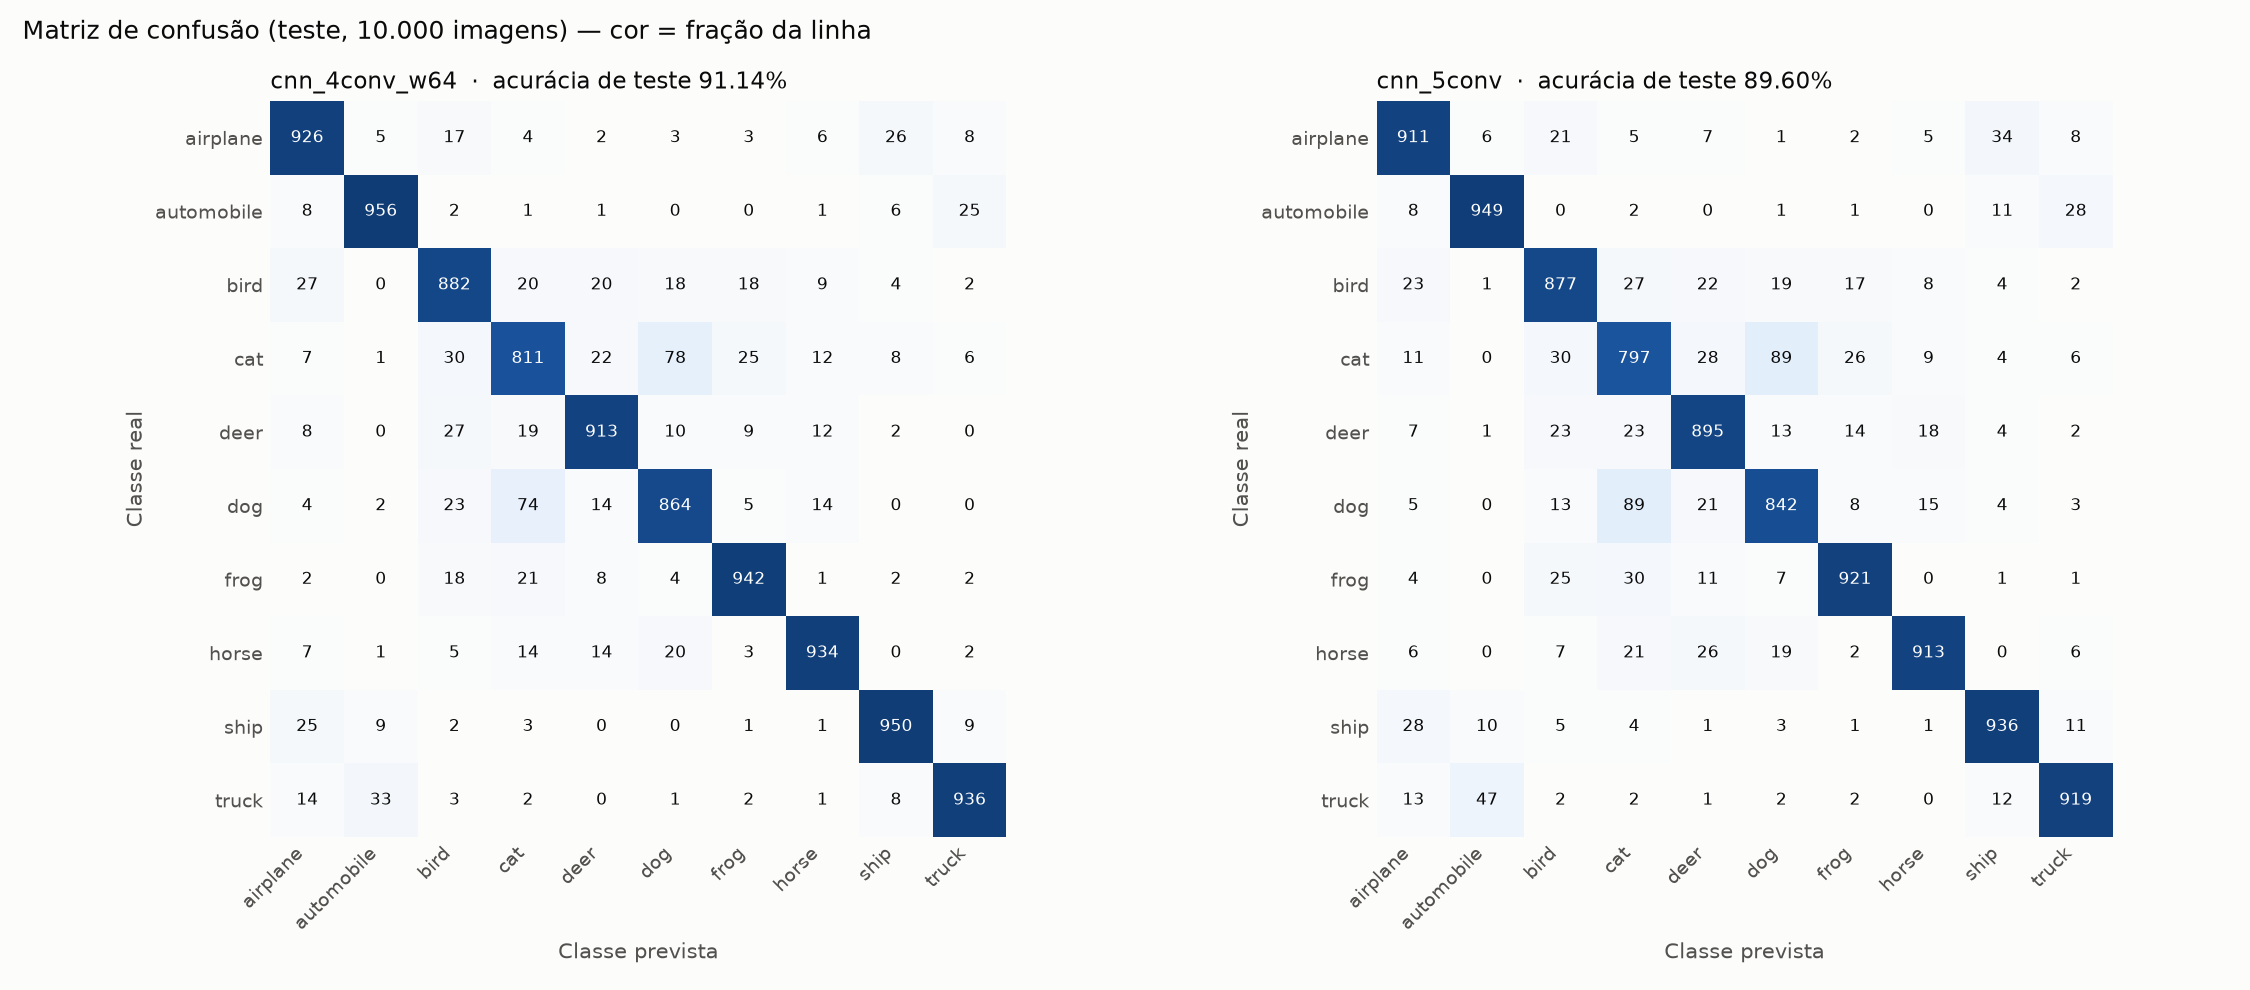
\includegraphics[width=\textwidth]{confusion_top2.png}
  \caption{Matrizes de confusão dos dois melhores modelos no conjunto de teste
           (\num{10000} imagens, \num{1000} por classe). Os números são contagens; a cor
           indica a fração de cada linha.}
  \label{fig:confusao}
\end{figure}

Os dois modelos erram de forma muito parecida. A maior confusão é entre \textit{cat} e
\textit{dog}, nos dois sentidos: 78 gatos classificados como cachorro e 74 cachorros como
gato em \code{cnn\_4conv\_w64}, contra 89 e 89 em \code{cnn\_5conv}. Em seguida vem
\textit{truck} classificado como \textit{automobile} (33 e 47 casos). Essas são classes
visualmente parecidas, ainda mais em $32\times32$ pixels. A classe mais difícil para os
dois modelos é \textit{cat} (\SI{81,1}{\percent} e \SI{79,7}{\percent}), e as mais fáceis
são \textit{automobile} e \textit{ship} (acima de \SI{93}{\percent}).

\begin{figure}[H]
  \centering
  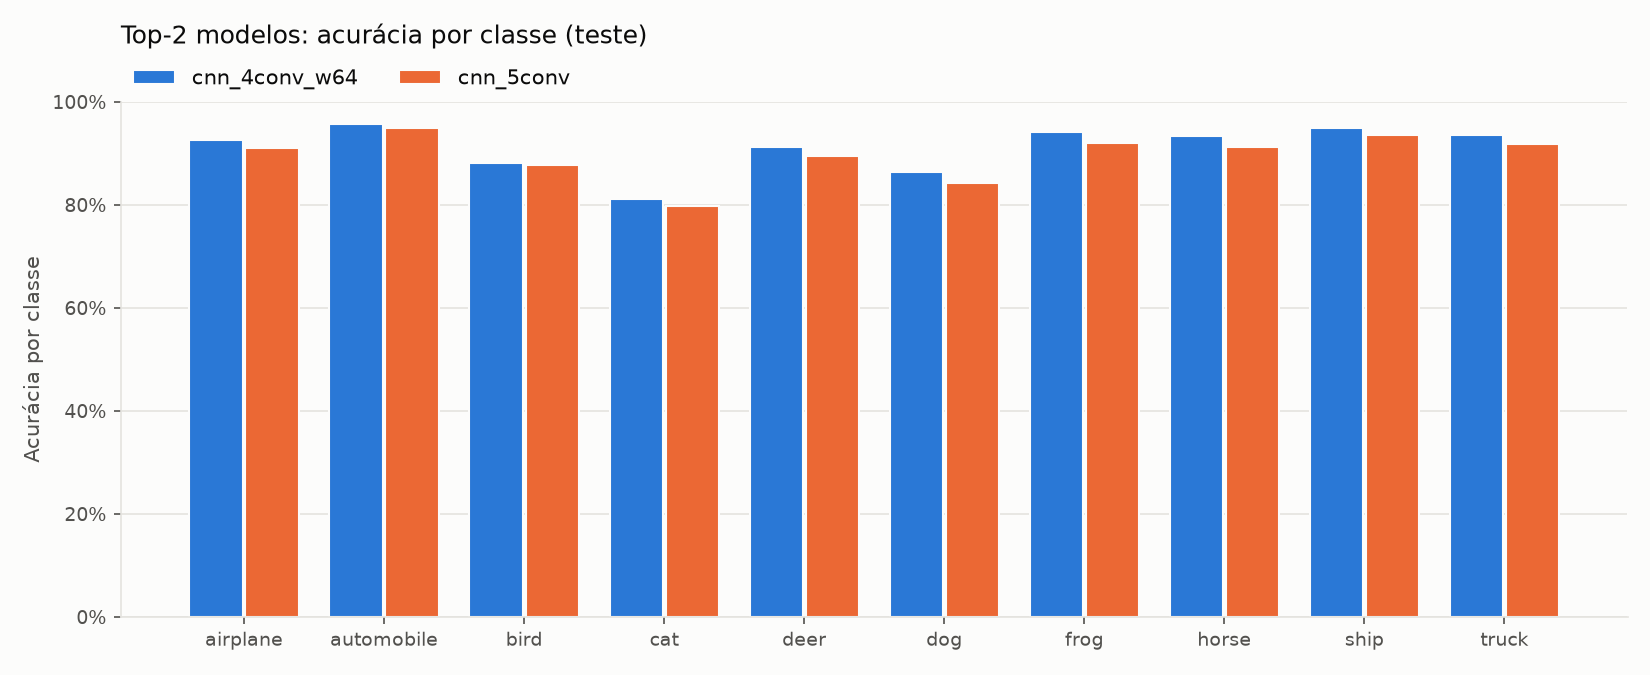
\includegraphics[width=0.9\textwidth]{per_class_top2.png}
  \caption{Acurácia por classe dos dois melhores modelos no conjunto de teste.}
  \label{fig:porclasse}
\end{figure}

\paragraph{Diferença entre os modelos.} A Tabela~\ref{tab:mcnemar} resume a comparação
pareada. Os dois modelos acertam as mesmas \num{8663} imagens e erram as mesmas
\num{589}; eles discordam em 748 imagens. Dessas, \code{cnn\_4conv\_w64} acerta 451 e
\code{cnn\_5conv} acerta 297.

\begin{table}[H]
  \centering
  \small
  \caption{Comparação pareada dos dois melhores modelos no conjunto de teste.}
  \label{tab:mcnemar}
  \begin{tabular}{lr}
    \toprule
    Acurácia de \code{cnn\_4conv\_w64}              & \SI{91,14}{\percent} \\
    Acurácia de \code{cnn\_5conv}                   & \SI{89,60}{\percent} \\
    Diferença                                       & $+\num{1,54}$ ponto percentual \\
    IC \SI{95}{\percent} (\textit{bootstrap})       & $[+\num{1,00};\ +\num{2,06}]$ \\
    Só \code{cnn\_4conv\_w64} acerta ($b$)          & 451 \\
    Só \code{cnn\_5conv} acerta ($c$)               & 297 \\
    Teste exato de McNemar                          & $p = \num{1,98e-8}$ \\
    \bottomrule
  \end{tabular}
\end{table}

Com $p < 0{,}05$ e um intervalo de confiança que não contém o zero, a diferença de
\num{1,54} ponto é estatisticamente significativa. Ela é pequena em termos práticos, mas
consistente: \code{cnn\_4conv\_w64} é melhor em todas as 10 classes
(Figura~\ref{fig:porclasse}), com as maiores vantagens em \textit{dog}, \textit{frog} e
\textit{horse} (cerca de 2 pontos cada). Como os dois modelos têm quase o mesmo número de
parâmetros (1,69 M e 1,70 M), o resultado indica que, neste orçamento de parâmetros, uma
rede mais larga e menos profunda funciona melhor do que uma mais profunda e mais estreita.

\subsection{CNN versus MLP}

A Tabela~\ref{tab:cnnmlp} compara a melhor CNN com o melhor MLP.

\begin{table}[H]
  \centering
  \small
  \caption{Melhor CNN versus melhor MLP.}
  \label{tab:cnnmlp}
  \begin{tabular}{lrr}
    \toprule
                        & CNN (\code{cnn\_4conv\_w64}) & MLP (\code{mlp\_5\_1024-64}) \\
    \midrule
    Acurácia de teste   & \textbf{\SI{91,14}{\percent}} & \SI{69,82}{\percent} \\
    Parâmetros          & \textbf{\num{1686794}}        & \num{3844682} \\
    Épocas              & 90                            & 400 \\
    Tempo de treino     & \textbf{\SI{302}{s}}          & \SI{1032}{s} \\
    \bottomrule
  \end{tabular}
\end{table}

A CNN acerta 21,3 pontos a mais usando 2,3 vezes menos parâmetros, menos épocas e menos
tempo de treino (McNemar, $p < 10^{-10}$). A Figura~\ref{fig:params} mostra que essa
vantagem vale para todos os modelos: qualquer CNN com três ou mais camadas
(\num{102602} parâmetros ou mais) supera todos os MLPs, inclusive o de 10,5 milhões de
parâmetros. O melhor MLP só supera a menor CNN (\code{cnn\_2conv}, \SI{69,2}{\percent}),
e para isso precisa de 175 vezes mais parâmetros.

\begin{figure}[H]
  \centering
  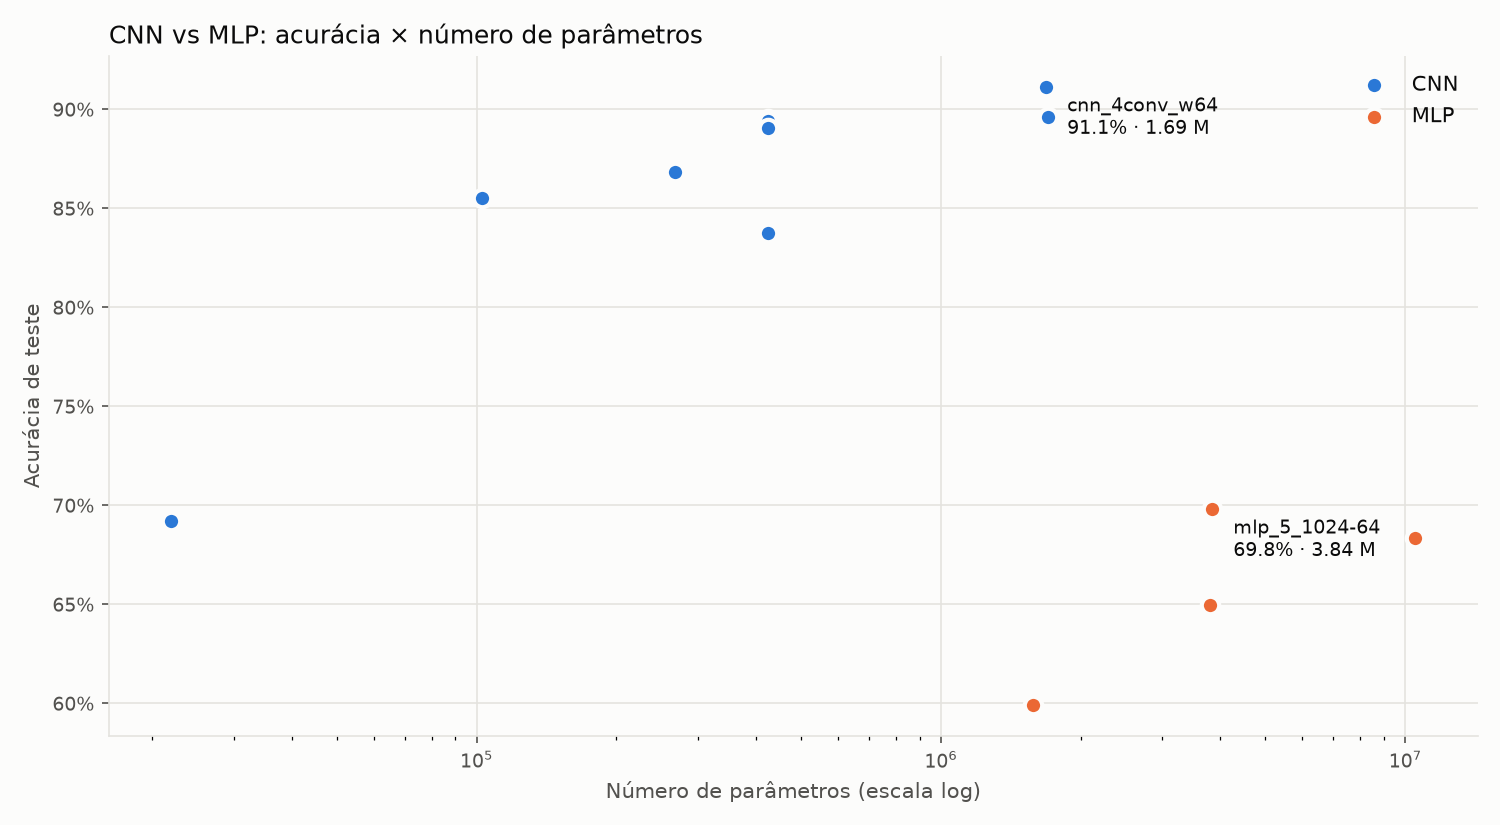
\includegraphics[width=0.9\textwidth]{acc_vs_params.png}
  \caption{Acurácia de teste em função do número de parâmetros (escala logarítmica).}
  \label{fig:params}
\end{figure}

A diferença vem da arquitetura. Na CNN, os mesmos filtros pequenos são aplicados em todas
as posições da imagem: a rede reconhece um padrão (uma borda, um olho, uma roda) onde quer
que ele apareça, e o \textit{pooling} torna a resposta tolerante a pequenos deslocamentos.
O MLP achata a imagem e liga cada pixel a pesos próprios, perdendo a estrutura espacial;
um objeto deslocado alguns pixels vira, para ele, uma entrada totalmente diferente. Por
isso o MLP precisa de muito mais parâmetros e exemplos para aprender a mesma coisa, e o
aumento de dados por deslocamento, que ajuda muito a CNN, torna o aprendizado do MLP mais
lento.

As confusões do MLP são as mesmas da CNN, mas muito mais frequentes: 230 cachorros
classificados como gato, 153 gatos como cachorro e 119 automóveis como caminhão. A
acurácia por classe do MLP vai de \SI{54,8}{\percent} (\textit{dog}) a
\SI{83,9}{\percent} (\textit{ship}).

\subsection{Efeito do número de épocas}
\label{sec:epocas}

Todos os modelos foram treinados primeiro por 30 épocas e depois por 90. Os MLPs também
foram treinados por 400 épocas. A Tabela~\ref{tab:epocas} mostra a acurácia de teste em
cada caso.

\begin{table}[H]
  \centering
  \small
  \caption{Acurácia de teste (\%) em função do número de épocas de treino.}
  \label{tab:epocas}
  \begin{tabular}{lrrr}
    \toprule
    Modelo & 30 épocas & 90 épocas & 400 épocas \\
    \midrule
    \code{cnn\_4conv\_w64}    & 90,08 & 91,14 & -- \\
    \code{cnn\_5conv}         & 87,74 & 89,60 & -- \\
    \code{cnn\_4conv}         & 87,31 & 89,54 & -- \\
    \code{cnn\_4conv\_nodrop} & 87,95 & 89,41 & -- \\
    \code{cnn\_4conv\_adamw}  & 87,09 & 89,05 & -- \\
    \code{cnn\_3conv\_k5}     & 84,93 & 86,83 & -- \\
    \code{cnn\_3conv}         & 81,76 & 85,54 & -- \\
    \code{cnn\_4conv\_noaug}  & 83,28 & 83,75 & -- \\
    \code{cnn\_2conv}         & 64,75 & 69,23 & -- \\
    \midrule
    \code{mlp\_5\_1024-64}    & 55,47 & 62,50 & 69,82 \\
    \code{mlp\_2x2048}        & 55,34 & 61,21 & 68,34 \\
    \code{mlp\_3\_1024-256}   & 52,47 & 57,97 & 64,96 \\
    \code{mlp\_1x512}         & 53,99 & 56,77 & 59,94 \\
    \bottomrule
  \end{tabular}
\end{table}

As CNNs grandes ganharam de 1 a 2 pontos de 30 para 90 épocas, e suas perdas de validação
se estabilizam no fim do treino. A exceção é \code{cnn\_4conv\_noaug}, que ganhou só
\num{0,5} ponto: sem aumento de dados, as épocas extras servem apenas para decorar o
conjunto de treino. Os MLPs ganharam mais (de cerca de 3 a 7 pontos a cada etapa), porque
estavam subajustados: sua perda de treino ficava acima da de validação. Com 400 épocas,
o melhor MLP (\code{mlp\_5\_1024-64}) parece ter convergido, já que sua perda de treino
cruza a de validação no fim. O \code{mlp\_1x512} se estabiliza em torno de
\SI{60}{\percent}, um limite da sua capacidade. A seleção dos dois melhores modelos e a
conclusão da comparação CNN versus MLP são as mesmas com 30, 90 ou 400 épocas.

% ---------------------------------------------------------------------------
\section{Conclusão}

\begin{itemize}
  \item A melhor rede foi \code{cnn\_4conv\_w64}, uma CNN de quatro camadas
        convolucionais com largura base 64, com \SI{91,14}{\percent} de acurácia de teste e 1,7
        milhão de parâmetros.
  \item Ela supera a segunda melhor (\code{cnn\_5conv}) por \num{1,54} ponto, com
        diferença estatisticamente significativa ($p \approx \num{2e-8}$) e vantagem em
        todas as classes. Os dois modelos confundem principalmente \textit{cat} e
        \textit{dog}.
  \item Profundidade até quatro camadas, largura e aumento de dados foram os fatores
        mais importantes. \textit{Dropout} e a escolha do otimizador tiveram pouco efeito.
  \item O melhor MLP chegou a \SI{69,82}{\percent} mesmo com 400 épocas, 21 pontos abaixo
        da melhor CNN e com 2,3 vezes mais parâmetros. Para imagens, o compartilhamento de
        pesos e a estrutura espacial das convoluções são muito mais eficientes do que
        camadas totalmente conectadas.
\end{itemize}

\paragraph{Limitações.} Cada configuração foi treinada uma única vez, com uma semente;
diferenças pequenas entre modelos do meio do \textit{ranking} (como entre
\code{cnn\_4conv}, \code{cnn\_4conv\_nodrop} e \code{cnn\_4conv\_adamw}) podem estar dentro
da variação entre execuções. Os MLPs foram avaliados apenas com aumento de dados; versões
sem o recorte aleatório poderiam convergir mais rápido.

\paragraph{Reprodutibilidade.} O código está em \code{src/}. Os resultados deste
relatório foram gerados com:
\begin{verbatim}
uv run python src/run_experiments.py --epochs 90 --out results_90ep
uv run python src/run_experiments.py --epochs 400 --out results_mlp400 \
    --only mlp_1x512 mlp_3_1024-256 mlp_2x2048 mlp_5_1024-64
uv run python src/run_experiments.py --merge results_90ep results_mlp400 \
    --out results_final
\end{verbatim}

\end{document}
